% Options for packages loaded elsewhere
\PassOptionsToPackage{unicode}{hyperref}
\PassOptionsToPackage{hyphens}{url}
%
\documentclass[
]{article}
\usepackage{amsmath,amssymb}
\usepackage{lmodern}
\usepackage{ifxetex,ifluatex}
\ifnum 0\ifxetex 1\fi\ifluatex 1\fi=0 % if pdftex
  \usepackage[T1]{fontenc}
  \usepackage[utf8]{inputenc}
  \usepackage{textcomp} % provide euro and other symbols
\else % if luatex or xetex
  \usepackage{unicode-math}
  \defaultfontfeatures{Scale=MatchLowercase}
  \defaultfontfeatures[\rmfamily]{Ligatures=TeX,Scale=1}
\fi
% Use upquote if available, for straight quotes in verbatim environments
\IfFileExists{upquote.sty}{\usepackage{upquote}}{}
\IfFileExists{microtype.sty}{% use microtype if available
  \usepackage[]{microtype}
  \UseMicrotypeSet[protrusion]{basicmath} % disable protrusion for tt fonts
}{}
\makeatletter
\@ifundefined{KOMAClassName}{% if non-KOMA class
  \IfFileExists{parskip.sty}{%
    \usepackage{parskip}
  }{% else
    \setlength{\parindent}{0pt}
    \setlength{\parskip}{6pt plus 2pt minus 1pt}}
}{% if KOMA class
  \KOMAoptions{parskip=half}}
\makeatother
\usepackage{xcolor}
\IfFileExists{xurl.sty}{\usepackage{xurl}}{} % add URL line breaks if available
\IfFileExists{bookmark.sty}{\usepackage{bookmark}}{\usepackage{hyperref}}
\hypersetup{
  pdftitle={Relatório de Planejamento e Análise de Experimentos},
  pdfauthor={Clevia Bento de Oliveira},
  hidelinks,
  pdfcreator={LaTeX via pandoc}}
\urlstyle{same} % disable monospaced font for URLs
\usepackage[margin=1in]{geometry}
\usepackage{color}
\usepackage{fancyvrb}
\newcommand{\VerbBar}{|}
\newcommand{\VERB}{\Verb[commandchars=\\\{\}]}
\DefineVerbatimEnvironment{Highlighting}{Verbatim}{commandchars=\\\{\}}
% Add ',fontsize=\small' for more characters per line
\usepackage{framed}
\definecolor{shadecolor}{RGB}{248,248,248}
\newenvironment{Shaded}{\begin{snugshade}}{\end{snugshade}}
\newcommand{\AlertTok}[1]{\textcolor[rgb]{0.94,0.16,0.16}{#1}}
\newcommand{\AnnotationTok}[1]{\textcolor[rgb]{0.56,0.35,0.01}{\textbf{\textit{#1}}}}
\newcommand{\AttributeTok}[1]{\textcolor[rgb]{0.77,0.63,0.00}{#1}}
\newcommand{\BaseNTok}[1]{\textcolor[rgb]{0.00,0.00,0.81}{#1}}
\newcommand{\BuiltInTok}[1]{#1}
\newcommand{\CharTok}[1]{\textcolor[rgb]{0.31,0.60,0.02}{#1}}
\newcommand{\CommentTok}[1]{\textcolor[rgb]{0.56,0.35,0.01}{\textit{#1}}}
\newcommand{\CommentVarTok}[1]{\textcolor[rgb]{0.56,0.35,0.01}{\textbf{\textit{#1}}}}
\newcommand{\ConstantTok}[1]{\textcolor[rgb]{0.00,0.00,0.00}{#1}}
\newcommand{\ControlFlowTok}[1]{\textcolor[rgb]{0.13,0.29,0.53}{\textbf{#1}}}
\newcommand{\DataTypeTok}[1]{\textcolor[rgb]{0.13,0.29,0.53}{#1}}
\newcommand{\DecValTok}[1]{\textcolor[rgb]{0.00,0.00,0.81}{#1}}
\newcommand{\DocumentationTok}[1]{\textcolor[rgb]{0.56,0.35,0.01}{\textbf{\textit{#1}}}}
\newcommand{\ErrorTok}[1]{\textcolor[rgb]{0.64,0.00,0.00}{\textbf{#1}}}
\newcommand{\ExtensionTok}[1]{#1}
\newcommand{\FloatTok}[1]{\textcolor[rgb]{0.00,0.00,0.81}{#1}}
\newcommand{\FunctionTok}[1]{\textcolor[rgb]{0.00,0.00,0.00}{#1}}
\newcommand{\ImportTok}[1]{#1}
\newcommand{\InformationTok}[1]{\textcolor[rgb]{0.56,0.35,0.01}{\textbf{\textit{#1}}}}
\newcommand{\KeywordTok}[1]{\textcolor[rgb]{0.13,0.29,0.53}{\textbf{#1}}}
\newcommand{\NormalTok}[1]{#1}
\newcommand{\OperatorTok}[1]{\textcolor[rgb]{0.81,0.36,0.00}{\textbf{#1}}}
\newcommand{\OtherTok}[1]{\textcolor[rgb]{0.56,0.35,0.01}{#1}}
\newcommand{\PreprocessorTok}[1]{\textcolor[rgb]{0.56,0.35,0.01}{\textit{#1}}}
\newcommand{\RegionMarkerTok}[1]{#1}
\newcommand{\SpecialCharTok}[1]{\textcolor[rgb]{0.00,0.00,0.00}{#1}}
\newcommand{\SpecialStringTok}[1]{\textcolor[rgb]{0.31,0.60,0.02}{#1}}
\newcommand{\StringTok}[1]{\textcolor[rgb]{0.31,0.60,0.02}{#1}}
\newcommand{\VariableTok}[1]{\textcolor[rgb]{0.00,0.00,0.00}{#1}}
\newcommand{\VerbatimStringTok}[1]{\textcolor[rgb]{0.31,0.60,0.02}{#1}}
\newcommand{\WarningTok}[1]{\textcolor[rgb]{0.56,0.35,0.01}{\textbf{\textit{#1}}}}
\usepackage{longtable,booktabs,array}
\usepackage{calc} % for calculating minipage widths
% Correct order of tables after \paragraph or \subparagraph
\usepackage{etoolbox}
\makeatletter
\patchcmd\longtable{\par}{\if@noskipsec\mbox{}\fi\par}{}{}
\makeatother
% Allow footnotes in longtable head/foot
\IfFileExists{footnotehyper.sty}{\usepackage{footnotehyper}}{\usepackage{footnote}}
\makesavenoteenv{longtable}
\usepackage{graphicx}
\makeatletter
\def\maxwidth{\ifdim\Gin@nat@width>\linewidth\linewidth\else\Gin@nat@width\fi}
\def\maxheight{\ifdim\Gin@nat@height>\textheight\textheight\else\Gin@nat@height\fi}
\makeatother
% Scale images if necessary, so that they will not overflow the page
% margins by default, and it is still possible to overwrite the defaults
% using explicit options in \includegraphics[width, height, ...]{}
\setkeys{Gin}{width=\maxwidth,height=\maxheight,keepaspectratio}
% Set default figure placement to htbp
\makeatletter
\def\fps@figure{htbp}
\makeatother
\setlength{\emergencystretch}{3em} % prevent overfull lines
\providecommand{\tightlist}{%
  \setlength{\itemsep}{0pt}\setlength{\parskip}{0pt}}
\setcounter{secnumdepth}{-\maxdimen} % remove section numbering
\ifluatex
  \usepackage{selnolig}  % disable illegal ligatures
\fi

\title{Relatório de Planejamento e Análise de Experimentos}
\author{Clevia Bento de Oliveira}
\date{22/09/2021}

\begin{document}
\maketitle

\hypertarget{relatuxf3rio-referente-uxe0-anuxe1lise-de-um-banco-de-dados-em-dic-utilizando-parcela-subdividida.}{%
\section{Relatório referente à análise de um banco de dados em DIC,
utilizando parcela
subdividida.}\label{relatuxf3rio-referente-uxe0-anuxe1lise-de-um-banco-de-dados-em-dic-utilizando-parcela-subdividida.}}

\hypertarget{introduuxe7uxe3o}{%
\subsection{Introdução}\label{introduuxe7uxe3o}}

No experimento em parcelas subdivididas, as parcelas experimentais são
divididas em sub parcelas. São estudados dois ou mais fatores
simultaneamente, tais fatores são chamados primários, secundários e
assim por diante.

Os fatores primários são aleatorizados nas parcelas, os secundários nas
sub parcelas. O modelo linear para o experimento em parcelas
subdivididas no delineamento em blocos ao acaso\\
é dado por:

\emph{yijk = µ + τi + βj + eij + θk + γik + Ɛikj}\\
onde:

\begin{itemize}
\tightlist
\item
  µ é a média geral;
\item
  τi é o efeito do i-ésimo tratamento sobre a variável resposta;
\item
  βj é o efeito do j-ésimo bloco sobre a variável resposta;
\item
  eik é o resíduo aleatório à nível de parcelas;
\item
  θk é o efeito do k-ésimo sub-tratamento sobre a variável resposta;
\item
  γik é o efeito da interação do i-ésimo tratamento com o j-ésimo
  subtratamento sobre a variável resposta;
\item
  Ɛijk é o resíduo aleatório associado a observação yijk à nível de
  sub-parcelas.
\end{itemize}

Neste trabalho será analisado um banco de dados fictício de um
experimento em blocos casualizados, onde há 3 espécies diferentes de
cultivares (CULT1, CULT2 e CULT3), 4 tipos diferentes de irrigação
(irrigacao1,irrigacao2,irrigacao3 e irrigacao4) com 3 repetições em
blocos casualizados.

\hypertarget{objetivo}{%
\subsubsection{Objetivo:}\label{objetivo}}

Comparar se há diferença significativa de produção no plantio de
diferentes espécies de cultivares e diferentes tipos de irrigação.

\hypertarget{metodologia}{%
\subsubsection{Metodologia}\label{metodologia}}

Para esta análise será utilizado o pacote \texttt{ExpDes.pt} para obter
a ANOVA e demais resultados.

\hypertarget{visualizauxe7uxe3o-dos-10-primeiros-dados-do-banco-de-dados}{%
\subsubsection{Visualização dos 10 primeiros dados do Banco de
Dados}\label{visualizauxe7uxe3o-dos-10-primeiros-dados-do-banco-de-dados}}

\begin{longtable}[]{@{}llrr@{}}
\toprule
Cultivares & Irrigacao & Bloco & Prod \\
\midrule
\endhead
CULT1 & irrigacao1 & 1 & 66 \\
CULT1 & irrigacao1 & 2 & 64 \\
CULT1 & irrigacao1 & 3 & 76 \\
CULT1 & irrigacao2 & 1 & 70 \\
CULT1 & irrigacao2 & 2 & 67 \\
CULT1 & irrigacao2 & 3 & 83 \\
CULT1 & irrigacao3 & 1 & 63 \\
CULT1 & irrigacao3 & 2 & 61 \\
CULT1 & irrigacao3 & 3 & 69 \\
CULT1 & irrigacao4 & 1 & 57 \\
\bottomrule
\end{longtable}

\hypertarget{anuxe1lise-descritiva}{%
\subsubsection{Análise Descritiva}\label{anuxe1lise-descritiva}}

\begin{verbatim}
##  Cultivares      Irrigacao     Bloco        Prod   
##  CULT1:12   irrigacao1:9   Min.   :1   60     : 2  
##  CULT2:12   irrigacao2:9   1st Qu.:1   66     : 2  
##  CULT3:12   irrigacao3:9   Median :2   68     : 2  
##             irrigacao4:9   Mean   :2   69     : 2  
##                            3rd Qu.:3   70     : 2  
##                            Max.   :3   71     : 2  
##                                        (Other):24
\end{verbatim}

\begin{verbatim}
## tibble [36 x 4] (S3: tbl_df/tbl/data.frame)
##  $ Cultivares: Factor w/ 3 levels "CULT1","CULT2",..: 1 1 1 1 1 1 1 1 1 1 ...
##  $ Irrigacao : Factor w/ 4 levels "irrigacao1","irrigacao2",..: 1 1 1 2 2 2 3 3 3 4 ...
##  $ Bloco     : num [1:36] 1 2 3 1 2 3 1 2 3 1 ...
##  $ Prod      : Factor w/ 27 levels "57","59","60",..: 7 6 16 11 8 20 5 4 10 1 ...
\end{verbatim}

\hypertarget{visualizauxe7uxe3o-do-experimento}{%
\subsubsection{Visualização do
Experimento}\label{visualizauxe7uxe3o-do-experimento}}

Aqui vemos a Irrigação dado os Cultivares

\includegraphics{relatoriosubdMarkdown_files/figure-latex/unnamed-chunk-3-1.pdf}

Aqui vemos os Cultivares dada a Irrigação
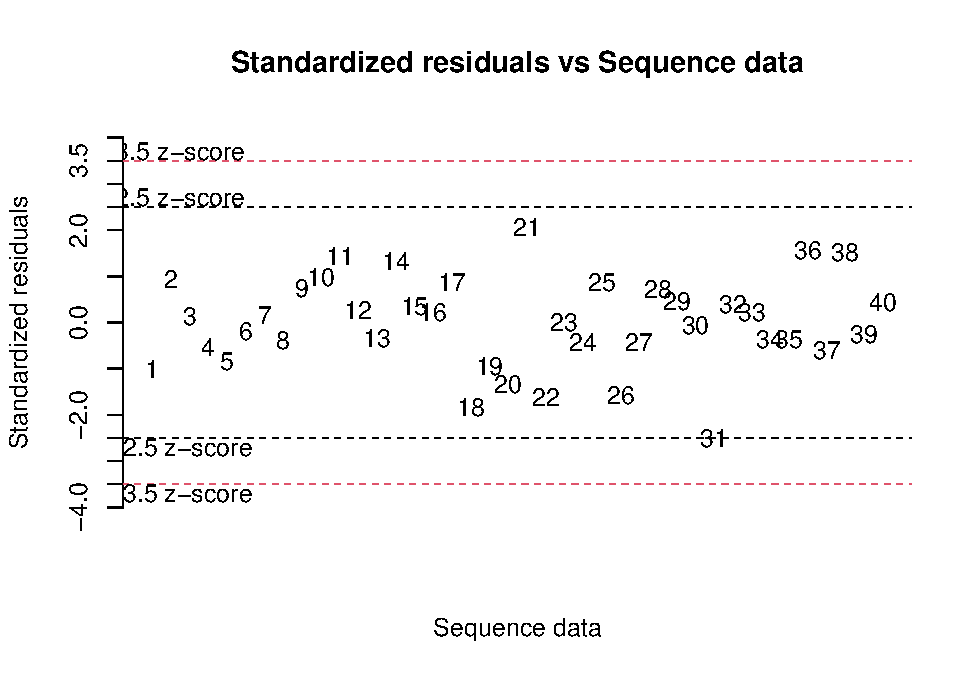
\includegraphics{relatoriosubdMarkdown_files/figure-latex/unnamed-chunk-4-1.pdf}

\hypertarget{teste-de-hipuxf3teses}{%
\subsubsection{Teste de Hipóteses}\label{teste-de-hipuxf3teses}}

\hypertarget{hipuxf3teses-que-queremos-testar}{%
\paragraph{Hipóteses que queremos
testar:}\label{hipuxf3teses-que-queremos-testar}}

H0: Não há diferença entre as irrigações em relação a produtividade.\\
H1: Há influência da irrigação na produtividade.

H0:Há diferença entre os blocos.\\
H1: Não há diferença entre os blocos.

H0: Não há diferença entre os cultivares na produtividade.\\
H1: Há diferença dos cultivares na produção.

H0: A interação entre os cultivares e irrigação não é significativa.\\
H1: A interação é significativa.

\begin{Shaded}
\begin{Highlighting}[]
\NormalTok{dados1.av }\OtherTok{=} \FunctionTok{aov}\NormalTok{(Prod }\SpecialCharTok{\textasciitilde{}}\NormalTok{  Cultivares}\SpecialCharTok{*}\NormalTok{Irrigacao }\SpecialCharTok{+} \FunctionTok{Error}\NormalTok{(Bloco}\SpecialCharTok{:}\NormalTok{Cultivares))}
\FunctionTok{summary}\NormalTok{(dados1.av)}
\end{Highlighting}
\end{Shaded}

\begin{verbatim}
## 
## Error: Bloco:Cultivares
##            Df Sum Sq Mean Sq F value Pr(>F)
## Cultivares  2   1408   704.2   1.476  0.503
## Residuals   1    477   477.0               
## 
## Error: Within
##                      Df Sum Sq Mean Sq F value   Pr(>F)    
## Cultivares            2    399   199.4   9.263  0.00131 ** 
## Irrigacao             3   2245   748.3  34.767 2.49e-08 ***
## Cultivares:Irrigacao  6   3563   593.9  27.596 6.33e-09 ***
## Residuals            21    452    21.5                     
## ---
## Signif. codes:  0 '***' 0.001 '**' 0.01 '*' 0.05 '.' 0.1 ' ' 1
\end{verbatim}

\hypertarget{anuxe1lise-de-resuxedduos}{%
\subsubsection{Análise de Resíduos}\label{anuxe1lise-de-resuxedduos}}

\begin{Shaded}
\begin{Highlighting}[]
\NormalTok{dados.avb }\OtherTok{=} \FunctionTok{aov}\NormalTok{(Prod }\SpecialCharTok{\textasciitilde{}}\NormalTok{ Cultivares}\SpecialCharTok{*}\NormalTok{Irrigacao }\SpecialCharTok{+}\NormalTok{ Bloco}\SpecialCharTok{*}\NormalTok{Cultivares}\SpecialCharTok{{-}}\NormalTok{Bloco)}
\FunctionTok{summary}\NormalTok{(dados.avb)}
\end{Highlighting}
\end{Shaded}

\begin{verbatim}
##                      Df Sum Sq Mean Sq F value   Pr(>F)    
## Cultivares            2   1687   843.4  39.186 8.17e-08 ***
## Irrigacao             3   2245   748.3  34.767 2.49e-08 ***
## Cultivares:Irrigacao  6   3564   593.9  27.596 6.33e-09 ***
## Cultivares:Bloco      3    597   199.1   9.252 0.000425 ***
## Residuals            21    452    21.5                     
## ---
## Signif. codes:  0 '***' 0.001 '**' 0.01 '*' 0.05 '.' 0.1 ' ' 1
\end{verbatim}

\begin{Shaded}
\begin{Highlighting}[]
\FunctionTok{par}\NormalTok{(}\AttributeTok{mfrow=}\FunctionTok{c}\NormalTok{(}\DecValTok{2}\NormalTok{,}\DecValTok{2}\NormalTok{))}
\FunctionTok{plot}\NormalTok{(dados.avb)}
\end{Highlighting}
\end{Shaded}

\includegraphics{relatoriosubdMarkdown_files/figure-latex/unnamed-chunk-6-1.pdf}

No segundo gráfico (superior à direita), estudamos a normalidade dos
resíduos. Quanto mais próximo da reta os pontos se distribuem mais
parecerá com uma distribuição normal, nesse caso os dados se distribuem
normalmente.

\hypertarget{teste-de-normalidade}{%
\subsubsection{Teste de Normalidade}\label{teste-de-normalidade}}

\begin{Shaded}
\begin{Highlighting}[]
\FunctionTok{shapiro.test}\NormalTok{(dados.avb}\SpecialCharTok{$}\NormalTok{residuals)}
\end{Highlighting}
\end{Shaded}

\begin{verbatim}
## 
##  Shapiro-Wilk normality test
## 
## data:  dados.avb$residuals
## W = 0.93821, p-value = 0.0447
\end{verbatim}

Podemos ver que o teste deu significativo, ou seja, os dados seguem uma
distribuição Normal.

\begin{verbatim}
## [1] "14" "5"  "32"
\end{verbatim}

\begin{verbatim}
## [1] "14" "32" "35"
\end{verbatim}

\includegraphics{relatoriosubdMarkdown_files/figure-latex/unnamed-chunk-8-1.pdf}

\begin{verbatim}
## 
##  Bartlett test of homogeneity of variances
## 
## data:  dados.avb$residuals and Irrigacao
## Bartlett's K-squared = 1.5667, df = 3, p-value = 0.667
\end{verbatim}

\begin{verbatim}
## 
##  Bartlett test of homogeneity of variances
## 
## data:  dados.avb$residuals and Cultivares
## Bartlett's K-squared = 0.059896, df = 2, p-value = 0.9705
\end{verbatim}

\hypertarget{anuxe1lise-utilizando-o-pacote-expdes.pt}{%
\subsubsection{\texorpdfstring{Análise utilizando o pacote
\texttt{ExpDes.pt}}{Análise utilizando o pacote ExpDes.pt}}\label{anuxe1lise-utilizando-o-pacote-expdes.pt}}

\begin{Shaded}
\begin{Highlighting}[]
\FunctionTok{require}\NormalTok{(ExpDes.pt)}
\FunctionTok{psub2.dbc}\NormalTok{(Cultivares, Irrigacao, Bloco, Prod, }\AttributeTok{quali =} \FunctionTok{c}\NormalTok{(}\ConstantTok{TRUE}\NormalTok{, }\ConstantTok{TRUE}\NormalTok{),}\AttributeTok{mcomp =} \StringTok{"tukey"}\NormalTok{,}
          \AttributeTok{fac.names =} \FunctionTok{c}\NormalTok{(}\StringTok{"Cultivares"}\NormalTok{, }\StringTok{"Irrigação"}\NormalTok{), }\AttributeTok{sigF =} \FloatTok{0.05}\NormalTok{)}
\end{Highlighting}
\end{Shaded}

\begin{verbatim}
## ------------------------------------------------------------------------
## Legenda:
## FATOR 1 (parcela):  Cultivares 
## FATOR 2 (subparcela):  Irrigação 
## ------------------------------------------------------------------------
## 
## ------------------------------------------------------------------------
## $`Quadro da analise de variancia\n------------------------------------------------------------------------\n`
##                      GL     SQ     QM     Fc   Pr(>Fc)    
## Cultivares            2 1686.7 843.36 26.750  0.004839 ** 
## Bloco                 2  722.7 361.36 11.462  0.022073 *  
## Erro a                4  126.1  31.53                     
## Irrigação             3 2244.8 748.25 67.175 < 2.2e-16 ***
## Cultivares*Irrigação  6 3563.5 593.92 53.319 < 2.2e-16 ***
## Erro b               18  200.5  11.14                     
## Total                35 8544.3                            
## ---
## Signif. codes:  0 '***' 0.001 '**' 0.01 '*' 0.05 '.' 0.1 ' ' 1
## 
## ------------------------------------------------------------------------
## CV 1 = 7.305333 %
## CV 2 = 4.342245 %
## 
## 
## 
## Interacao significativa: desdobrando a interacao
## ------------------------------------------------------------------------
## 
## Desdobrando  Cultivares  dentro de cada nivel de  Irrigação 
## ------------------------------------------------------------------------
##                                          GL          SQ          QM        Fc
## Cultivares : Irrigação irrigacao1   2.00000    4.666667    2.333333  0.143713
## Cultivares : Irrigação irrigacao2   2.00000 2546.000000 1273.000000 78.405474
## Cultivares : Irrigação irrigacao3   2.00000  480.888889  240.444444 14.809239
## Cultivares : Irrigação irrigacao4   2.00000 2218.666667 1109.333333 68.325064
## Erro combinado                     13.58219  220.521944   16.236111          
##                                     valor.p
## Cultivares : Irrigação irrigacao1  0.867436
## Cultivares : Irrigação irrigacao2         0
## Cultivares : Irrigação irrigacao3  0.000387
## Cultivares : Irrigação irrigacao4         0
## Erro combinado                             
## ------------------------------------------------------------------------
## 
## 
##  Cultivares dentro de Irrigação irrigacao1
## ------------------------------------------------------------------------
## De acordo com o teste F, as medias desse fator sao estatisticamente iguais.
## ------------------------------------------------------------------------
##   Niveis   Medias
## 1  CULT1 68.66667
## 2  CULT2 68.33333
## 3  CULT3 70.00000
## ------------------------------------------------------------------------
## 
##  Cultivares dentro de Irrigação irrigacao2
## ------------------------------------------------------------------------
## Teste de Tukey
## ------------------------------------------------------------------------
## Grupos Tratamentos Medias
## a     CULT3   112.3333 
##  b    CULT2   81.33333 
##  b    CULT1   73.33333 
## ------------------------------------------------------------------------
## 
##  Cultivares dentro de Irrigação irrigacao3
## ------------------------------------------------------------------------
## Teste de Tukey
## ------------------------------------------------------------------------
## Grupos Tratamentos Medias
## a     CULT2   81 
##  b    CULT3   67 
##  b    CULT1   64.33333 
## ------------------------------------------------------------------------
## 
##  Cultivares dentro de Irrigação irrigacao4
## ------------------------------------------------------------------------
## Teste de Tukey
## ------------------------------------------------------------------------
## Grupos Tratamentos Medias
## a     CULT2   100 
##  b    CULT3   73.33333 
##   c   CULT1   62.66667 
## ------------------------------------------------------------------------
## 
## 
## Desdobrando  Irrigação  dentro de cada nivel de  Cultivares 
## ------------------------------------------------------------------------
##                               GL        SQ         QM        Fc  valor.p
## Irrigação : Cultivares CULT1   3  205.5833   68.52778   6.15212 0.004577
## Irrigação : Cultivares CULT2   3 1531.3333  510.44444 45.825436        0
## Irrigação : Cultivares CULT3   3 4071.3333 1357.11111 121.83541        0
## Erro b                        18  200.5000   11.13889                   
## ------------------------------------------------------------------------
## 
## 
##  Irrigação dentro de Cultivares CULT1
## ------------------------------------------------------------------------
## Teste de Tukey
## ------------------------------------------------------------------------
## Grupos Tratamentos Medias
## a     irrigacao2      73.33333 
## ab    irrigacao1      68.66667 
##  b    irrigacao3      64.33333 
##  b    irrigacao4      62.66667 
## ------------------------------------------------------------------------
## ------------------------------------------------------------------------
## 
## 
##  Irrigação dentro de Cultivares CULT2
## ------------------------------------------------------------------------
## Teste de Tukey
## ------------------------------------------------------------------------
## Grupos Tratamentos Medias
## a     irrigacao4      100 
##  b    irrigacao2      81.33333 
##  b    irrigacao3      81 
##   c   irrigacao1      68.33333 
## ------------------------------------------------------------------------
## ------------------------------------------------------------------------
## 
## 
##  Irrigação dentro de Cultivares CULT3
## ------------------------------------------------------------------------
## Teste de Tukey
## ------------------------------------------------------------------------
## Grupos Tratamentos Medias
## a     irrigacao2      112.3333 
##  b    irrigacao4      73.33333 
##  b    irrigacao1      70 
##  b    irrigacao3      67 
## ------------------------------------------------------------------------
## ------------------------------------------------------------------------
\end{verbatim}

\hypertarget{conclusuxe3o}{%
\subsection{Conclusão}\label{conclusuxe3o}}

Pela análise de Variâncias as interações foram significativas.\\
Analisando os desdobramentos temos que:\\
Para a Irrigação 1, os Cultivares não apresentaram diferença
significatica.\\
Para a Irrigação 2, o Cultivar 3 teve melhor desempenho, seguido do
Cultivar 2.\\
Para a Irrigação 3, o Cultivar 2 teve melhor desempenho.\\
Para a Irrigação 4, o Cultivar 2 teve melhor desempenho. Com isso
podemos concluir que dentre os 3 Cultivares, o Cultivar 2 apresenta
melhores resultados\\
em relação ás Irrigações.

Para o Cultivar 1, a Irrigação 2 apresenta melhores resultados.\\
Para o Cultivar 2, a Irrigação 4 apresenta melhores resultados.\\
Para o Cultivar 3, a Irrigação 2 apresenta melhores resultados.\\
Podemos concluir que dentre as 4 Irrigações, a Irrigação 2 apresenta
melhores resultados\\
em relação aos Cultivares.

\end{document}
